\section{Quantum Computing}

Classical computers have been getting exponentially faster over the last 50 years, as observed by Moore's law \cite{Moore1965}. Still, it was suggested as early as 1982 that a classical computer may never be efficient at modeling a quantum mechanical system \cite{Feynman1982}. This is because of superposition (\cref{sub:Superposition}) and entanglement (\cref{sub:Entanglement}).

The idea of using a quantum computer is to make use of these very same properties that make a quantum system challenging to simulate, but to use them to one's advantage instead. If this would be possible, we can simulate new molecules and chemical reaction mechanisms, opening up the road to novel medicine \cite{Robert2021} and materials \cite{Ma2020}. 

\subsection{Superposition}\label{sub:Superposition}

Consider a single two level quantum system, quantum bit or 'qubit' $\ket{\psi}$, for example the spin of an electron, which we can define as a basis with basis states $\ket{0}$ (spin up) and $\ket{1}$ (spin down). According to quantum mechanics, this qubit can be in a superposition state \cite{Griffiths2004}:

\begin{equation}\label{eq:SuperPositionBasic}
	\ket{\psi}=a\ket{0}+b\ket{1},
\end{equation}

where $a,b \in \mathbb{C}$, where one will measure $\ket{0}$ (spin up in this example) with probability $|a|^2$ and and $\ket{1}$ (spin down) with $|b|^2$. Without loss of generality, we can let the variable $\theta$ keep track of the probability of measuring $\ket{0}$ or $\ket{1}$, and defining $\phi$ as the relatively phase between the two. This is powerful because we can plot the Hilbert space of the qubit on a unit sphere called the Bloch sphere representation \cite{Nielsen2011}

\begin{equation}\label{eq:BlochSphere}
	\ket{\psi} = 
	\cos{\frac{\theta}{2}} \ket{0} + e^{i \phi} \sin{\frac{\theta}{2}} \ket{1}
\end{equation}

This Bloch sphere is shown in \cref{fig:BlochSphere}. Classical binary bits are shown as well, which in this analogy occupy only the poles of the sphere, whereas the quantum state can be anywhere on this unit sphere. This is the first hint of the computational potential of a quantum computer. But to build a quantum computer, we are going to need more than one qubit. While we cannot easily graphically represent multi qubit states like for the Bloch sphere, we can still write them down, for which we will introduce the concept entanglement.

\begin{figure}
	\centering
	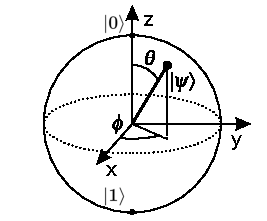
\includegraphics[width=.28\linewidth]{figures/BlochSphereCropped.pdf}
	\caption{The Bloch sphere representation. A classical bit can only be $\ket{0}$ or $\ket{1}$, whereas a qubit can occupy any point on the sphere with coordinates $\theta, \phi$. Figure adapted from \cite{Jones2012}.}
	\label{fig:BlochSphere}
\end{figure}

\subsection{Entanglement}\label{sub:Entanglement}

We will extend from 1 to 2 electrons. Now, they can be independently spin up $\ket{0}$ and down: $\ket{1}$, for a total of 4 basis states. Quantum physics teaches us this system can be in a superposition of all its basis states \cite{Nielsen2011}:

\begin{equation}\label{eq:TwoQubits}
	\ket{\psi_{2q}} = 
	\alpha_{00} \ket{00} + \alpha_{01} \ket{01} + \alpha_{10} \ket{10} + \alpha_{11} \ket{11}.
\end{equation}

Where $\ket{00}$ is shorthand notation for both qubits being in the spin up state, etc. In general, the size of the Hilbert space will grow as $2^N$ for $N$ qubits \cite{Henriet2020,Nielsen2011}. For $N=300$, this is already larger than the estimated amount of particles in the observable universe at some $\sim 10^{80}$. However, to really access the full Hilbert space, the qubits need to be entangled. These are an inherent quantum feature, having no classical analogue. One of the most instructive examples of an entangled state is 

\begin{equation}\label{eq:Entangled}
	\ket{\Phi^+} = \frac{1}{\sqrt{2}} \ket{00}+ \frac{1}{\sqrt{2}} \ket{11}
\end{equation}

This is one of the so called Bell states \cite{Nielsen2011} and it is said to be entangled: upon measuring just one of the qubits we immediately know the state of the other qubit as well. This implies the qubits are correlated and cannot be described as a product of independent single qubits. In the operation of a quantum computer, entanglement is a crucial step during the computation stage \cite{Henriet2020}. 

\section{The NISQ Era}

Constructing a quantum computer is challenging because apart from full control over each qubit, they should ideally not interact with the environment at all, as this can change their quantum state. This is effect is known as decoherence \cite{DiVincenzo2000}.

Decoherence errors can be corrected but this requires a significant overhead in the available number of qubits and is unachievable in the near term \cite{Peres1985,Ladd2010}. Therefore, quantum computing is currently in the \ac{NISQ} \cite{Preskill2018}. Noisy refers to the notion that the measured probability amplitudes of the qubits may be slightly different than theoretically expected. The amount of noise can be quantified in a number known as the fidelity, a number between 0 and 1 where 1 means perfect control and zero noise. 

During the \ac{NISQ} era, the algorithms that run on quantum computers should be optimized for finite coherence times and fidelities. One algorithm proposed by \cite{Peruzzo2014} is thought to run especially well on non error-corrected hardware, so we will briefly describe its basic principle here \cite{McClean2016}. 

\subsection{The Variational Quantum Eigensolver}

The \ac{VQE} is an hybrid quantum algorithm: by making use of classical hardware it aims to reduce the amount of quantum gates needed, which is advantageous on NISQ era hardware with finite coherence times \cite{McClean2016}. Essentially, \ac{VQE} tries to find approximately the ground state energy of an atom or molecule according to the variational principle \cite{Griffiths2004}, which states that the expectation value of a given Hamiltonian $\mathcal{H}$ will always be an upper bound for the ground state energy $E_g$:

\begin{equation}\label{eq:VariationalPrinciple}
	\left\langle \mathcal{H} \right\rangle = \bra{\Psi}\mathcal{H} \ket{\Psi} \geq E_g.
\end{equation}

This is equivalent to finding the eigenvalues of the matrix $\mathcal{H}$. Even for a relatively simple molecules, $\mathcal{H}$ quickly becomes large and the task op diagonalizing it intractable, at least for a classical computer. In \ac{VQE}, $\mathcal{H}$ is not directly diagonalized but the Hamiltonian is prepared in a quantum co-processor or quantum processing unit (QPU) \cite{Henriet2020,Peruzzo2014}, taking advantage of the large Hilbert state of the quantum hardware. 

Given an ansatz $\theta$, a trial state $\ket{\Psi(\theta)}$ is prepared. The Hamiltonian is written in the form of a sum of Pauli strings: $P_{\alpha}$ with weights $h_{\alpha}$ \cite{McClean2016,Moll2018}

\begin{equation}\label{eq:PauliDecomposition}
	\mathcal{H} = \sum_{\alpha} h_{\alpha} P_{\alpha}
\end{equation}

\begin{figure}
	\centering
	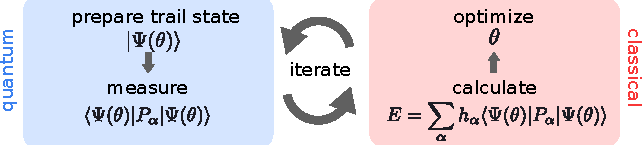
\includegraphics[width=0.75\linewidth]{figures/VQE.pdf}
	\caption{The \ac{VQE} visualized. Meant to run on a hybrid quantum computer, starting from an ansatz for the wave function it is prepared and the expectation function of its energy measured by a series of measurements on the QPU. Next, a CPU uses a non-linear optimization to find a new ansatz that will decrease the expectation value of $\mathcal{H}$. Iterated until convergence. Figure adapted from \cite{Moll2018}}
	\label{fig:VQE}
\end{figure}

The Pauli string is essentially a tensor product of Pauli spin matrices, the definition is given in appendix \ref{ch:PauliExpectation}. Because of the decomposition in Pauli strings, estimating the various terms of the Hamiltonian $\bra{\Psi} P_{\alpha} \ket{\Psi}$ boils down to measuring populations of individual qubits, this is explained in appendix \ref{ch:PauliExpectation}. The total expectation value of the Hamiltonian is obtained by summing over contributions of the Pauli strings. This is done on classical hardware. Subsequently, a non-linear optimizer is run to minimize the energy using a new trial state, and the cycle repeats \cite{Moll2018}. The algorithm is visualized in \cref{fig:VQE}. The quantum and classical parts of the algorithms feed into each other, therefore \ac{VQE} is referred to as a hybrid algorithm. 


\section{Hardware Implementation}

Now that we know what type of algorithm we aim to run, we will discuss the choice of the quantum hardware implementation. A list of criteria for this was formulated by \cite{DiVincenzo2000}. Based on this, several quantum computer realizations have been proposed \cite{Ladd2010}. Examples include: infrared photons \cite{Matthews2009},  trapped ions \cite{Benhelm2008,Schindler2013}, electron spins \cite{Press2008} and superconducting currents \cite{DiCarlo2009,Arute2019}. 

\subsection{Neutral Atoms}

At TU/e, we aim to build a quantum computer based on qubit states encoded in the electronic states of neutral atoms. The atoms are assembled in arbitrary geometries using laser cooling an trapping techniques. This technique is thought to easily scale to higher number of qubits by increasing the trapping laser power \cite{Henriet2020}. 

The atoms are held in place by optical dipole traps \cite{Chu1986}, each trap is non-deterministically loaded with single atoms \cite{Schlosser2001}. Multiple dipole traps spaced a couple of micro meters from each other are made using holography techniques \cite{Bergamini2004}. Quantum gates and measurements are performed by exciting to Rydberg states and applying Rabi pulses \cite{Levine2018,Madjarov2020}. Qubit states are detected using probe laser pules. A schematic overview of the different steps in neutral atom quantum computing are shown in \cref{fig:ComputingSteps}.

\begin{figure}
	\centering
	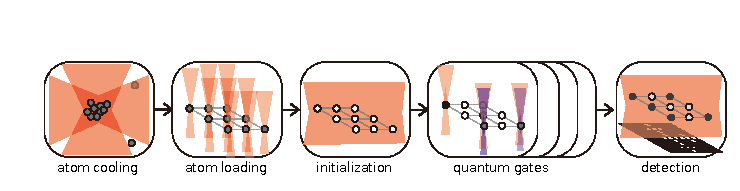
\includegraphics[width=\linewidth]{figures/ComputingSteps.pdf}
	\caption{A schematic drawing of the different steps involved in running a QPU based on neutral atoms in optical tweezers, excited to Rydberg states. Starting with a cloud of ultracold atom, the atoms are loaded in an array and the qubits are initialized. Gate operations, as well as readout measurements are performed by applying various laser pulses. Figure from \cite{Wu2021}.}
	\label{fig:ComputingSteps}
\end{figure}

\section{This Thesis}

In a collaboration with the \textit{Schreck} group at the University of Amsterdam, we aim to realize a \ac{NISQ} era quantum processing unit. The machine will feature ultracold strontium atoms trapped in arrays of tightly focused laser beams or optical tweezers. This platform has recently shown to achieve high-fidelity quantum gates and measurements \cite{Madjarov2020}. The purpose of this thesis is to give an insight in the first steps carried out at Eindhoven University of Technology towards this goal, which at the time of writing mostly concerns the first two steps in \cref{fig:ComputingSteps}. In order to do this this work is organized in the following way:

\begin{itemize}
	\setlength\itemsep{0em}
	\item Background information about laser cooling and trapping techniques, as well as for strontium specifically is presented in \cref{ch:coolingtrapping}. 

	\item How we make an optical tweezer inside a vacuum chamber is described in \cref{ch:tweezer}. 

	\item Chapter \ref{ch:arrays} elaborates on how to make arrays in arbitrary geometries using holography techniques.

	\item Finally, in \cref{ch:implementation} we describe how to implement the setup in an ultracold atoms experiment.
\end{itemize}










